%************************************************
\chapter{Prove dinamico-meccaniche}\label{chp:DinamicoMeccaniche}
%************************************************
Consistono nell'imporre al materiale una storia di deformazione periodica nel tempo.
Ad esempio:
\begin{equation}
\epsilon(t) = \bar{\epsilon}\sin(\omega t)
\end{equation}
Assomiglia ad una prova di fatica per i metalli, ma ha tutt'altro significato.

Bastano alcuni minuti di sollecitazione a $\epsilon(t)$ per ottenere i dati caratteristici del materiale. Inoltre, in questo caso si controlla la deformazione e il materiale non si rompe.

I dati che si ottengono sono:
\begin{equation}
\begin{split}
\sigma(t) &= \epsilon(0)E(t) + \int_0^t{E(t-\tau)\dot{\epsilon}(s)\,ds}\\
E(t) &= E_{\infty} + \Delta E(t)
\end{split}
\end{equation}
Se il materiale è fluido viscoelastico allora $E_{\infty} = 0$, altrimenti $E_{\infty} > 0$.
Mente $\Delta E(t) \underrightarrow{t \rightarrow \infty} 0$.
Allora:
\begin{equation}
\begin{split}
\sigma(t) &= \epsilon(0)(E_{\infty} + \Delta E(t)) + \int_0^t{(E_{\infty} + \Delta E(t-s)) \dot{\epsilon}(s)\,ds}\\
&= \epsilon(0)E_{\infty} + \epsilon(0)\Delta E(t) + \int_0^t{E_{\infty}\dot{\epsilon}(s)\,ds} +  \int_0^t{\Delta E(t-s) \dot{\epsilon}(s)\,ds}\\
&= \epsilon(0)E_{\infty} + \epsilon(0)\Delta E(t) + E_{\infty}(\epsilon(t) - \epsilon(0)) + \int_t^0{\Delta E(\tau) \dot{\epsilon}(t-\tau)\,-d\tau}\\
&= \epsilon(0)\Delta E(t) + E_{\infty}\epsilon(t) + \int_0^t{\Delta E(s) \dot{\epsilon}(t-s)\,ds}\\
\end{split}
\end{equation}
Imponendo che $\epsilon(t) = \bar{\epsilon}\sin(\omega t)$ allora:
\begin{equation}
\begin{split}
\sigma(t) &= E_{\infty} \bar{\epsilon}\sin(\omega t) + \int_0^t{\Delta E(s)\omega\bar{\epsilon}\cos(\omega(t-s))\,ds}\\
&= E_{\infty} \bar{\epsilon}\sin(\omega t) + \omega\bar{\epsilon}\int_0^t{\Delta E(s) \left[\cos(\omega t)\cos(\omega s) + \sin(\omega t)\sin(\omega s)\right]\,ds}\\
&= E_{\infty} \bar{\epsilon}\sin(\omega t) + \omega\bar{\epsilon}\int_0^t{\Delta E(s) \cos(\omega t)\cos(\omega s)\,ds} +\\
&\omega\bar{\epsilon}\int_0^t{\Delta E(s)\sin(\omega t)\sin(\omega s)\,ds}\\
&= E_{\infty} \bar{\epsilon}\sin(\omega t) + \omega\bar{\epsilon}\cos(\omega t)\int_0^t{\Delta E(s) \cos(\omega s)\,ds} +\\
&\omega\bar{\epsilon}\sin(\omega t)\int_0^t{\Delta E(s)\sin(\omega s)\,ds}\\
&= \bar{\epsilon}\left[E_{\infty} + \omega\int_0^t{\Delta E(s)\sin(\omega s)\,ds}\right]\sin(\omega t) +\\
&\bar{\epsilon}\left[\omega\int_0^t{\Delta E(s)\cos(\omega s)\,ds}\right]\cos(\omega t)
\end{split}
\end{equation}
Sarebbe la storia di deformazione è sinusoidale, non è detto che la storia di sforzo lo sia.
\begin{equation}
\begin{split}
\int_0^t{\Delta E(s)\sin(\omega s)\,ds} \quad \overrightarrow{t \rightarrow \infty} \quad \exists \int_0^t{\Delta E(s)\sin(\omega s)\,ds} < \infty\\
\int_0^t{\Delta E(s)\cos(\omega s)\,ds} \quad \overrightarrow{t \rightarrow \infty} \quad \exists \int_0^t{\Delta E(s)\cos(\omega s)\,ds} < \infty\\
\end{split}
\end{equation}
\begin{equation}
\sigma(t) = \bar{\epsilon}\left\lbrace\underbrace{\left[E_{\infty} + \omega\int_0^t{\Delta E(s)\sin(\omega s)\,ds}\right]}_{E'(\omega)}\sin(\omega t) + \underbrace{\left[\omega\int_0^t{\Delta E(s)\cos(\omega s)\,ds}\right]}_{E"(\omega)}\cos(\omega t)\right\rbrace
\end{equation}
Da cui:
\begin{equation}
\begin{cases}
\sigma(t) &= \bar{\epsilon} E'(\omega)\sin(\omega t) + \bar{\epsilon} E"(\omega)\cos(\omega t)\\
E'(\omega) &:=\textup{ Modulo conservativo}\\
E"(\omega) &:=\textup{ Modulo dissipativo}
\end{cases}
\end{equation}
Si riesce a vedere quanto il materiale è in grado di mantenere energia rispetto a quanto ne dissipi.

\begin{description}
\item[Modulo conservativo] parte in fase con la sollecitazione, rappresenta la capacità del materiale di conservare energia.
\item[Modulo dissipativo] parte in contro fase con la sollecitazione, rappresenta la capacità del materiale a dissipare energia. 
\end{description}

\section{Come viene realizzata la prova?}
Se la forzate è definita come: $\epsilon(t) = \bar{\epsilon}\sin(\omega t)$ allora lo sforzo può essere visto come: $\sigma(t) = \bar{\sigma}\sin(\omega t + \delta)$. Da cui:
\begin{equation}
\begin{split}
\sigma(t) &= \bar{\sigma}\left(\sin(\omega t)\cos(\delta) + \cos(\omega t)\sin(\delta)\right) =\\
&= \underbrace{(\bar{\sigma}\cos(\delta))}_{\bar{\epsilon}E'}\sin(\omega t) + \underbrace{(\bar{\sigma}\sin(\delta))}_{\bar{\epsilon}E"}\cos(\omega t)\\
\begin{cases}
E' &=\frac{\bar{\sigma}}{\bar{\epsilon}}\cos(\delta)\\
E" &=\frac{\bar{\sigma}}{\bar{\epsilon}}\sin(\delta)
\end{cases}
\end{split}
\end{equation}

\begin{figure}
\centering
\subfloat[][\emph{Componente conservativa}\label{fig:ComponenteConservativa}]
{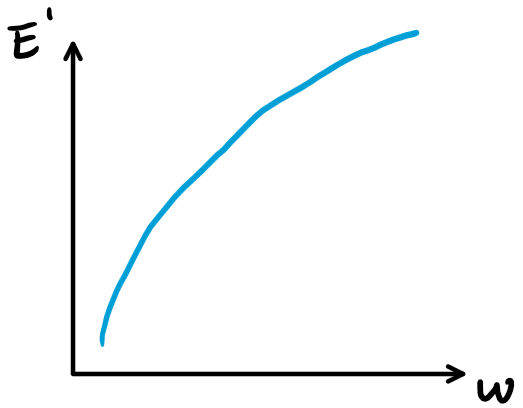
\includegraphics[width = 0.4\textwidth]{gfx/ComponenteConservativa}}\quad
\subfloat[][\emph{Componente dissipativa}\label{fig:ComponenteDissipativa}]
{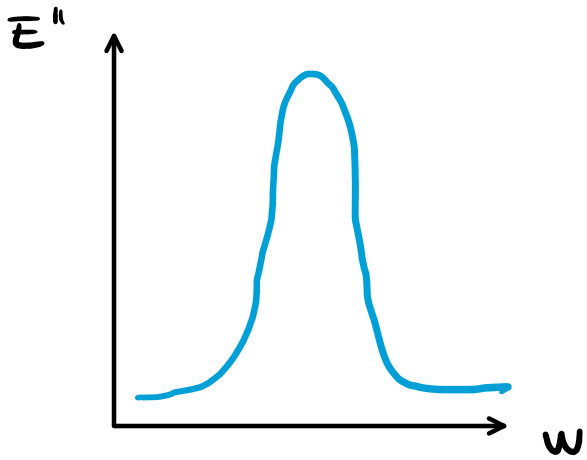
\includegraphics[width = 0.4\textwidth]{gfx/ComponenteDissipativa}}\\
\subfloat[][\emph{Combinazione sul materiale della deformazione e sforzo nella prova dinamica}\label{fig:Combinazione}]
{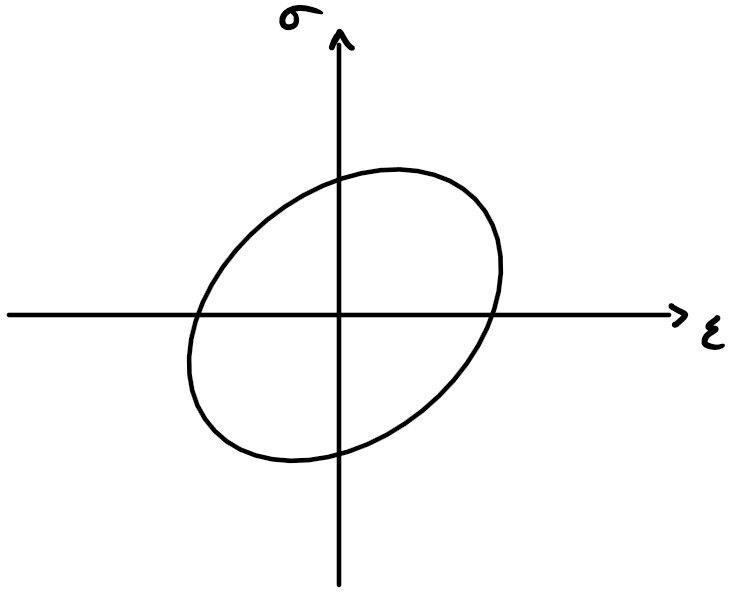
\includegraphics[width = 0.5\textwidth]{gfx/Combinazione}}
\caption{Componenti della prova dinamico-meccanica}
\label{fig:ComponentiProva}
\end{figure}

Dalla figura \ref{fig:ComponentiProva}, si osserva che le componenti hanno comportamento diverso tra loro.
\begin{description}
\item[Componente conservativa $E'$] ha un andamento crescente al crescere della frequenza della prova.
\item[Componente dissipativa $E"$] ha un andamento a campana, dunque per basse e alte frequenza tende a zero, ha un picco per frequenze intermedie.
\end{description}

Allora:
\begin{equation}
\begin{split}
\epsilon(t) &= \bar{\epsilon}\sin(\omega t) \doteq \omega \bar{\epsilon}\cos(\omega t)\\
\sigma(t) &= \bar{\sigma}\sin(\omega t + \delta)
\end{split}
\end{equation}
In termini energetici:
\begin{equation}
\begin{split}
W &= \int_{ciclo}\sigma\,d\epsilon\\
&= \int_t^{t+\frac{2\pi}{\omega}}{\sigma \frac{d\epsilon}{ds}\,ds}\\
W &= \int_t^{t+\frac{2\pi}{\omega}}{\bar{\sigma}\sin(\omega t + \delta) \cdot \omega \bar{\epsilon}\cos(\omega s)\,ds}\\
W &= \bar{\sigma} \bar{\epsilon}\omega\int_t^{t+\frac{2\pi}{\omega}}{\cos(\omega s)\left[\sin(\omega s)\cos(\delta) + \cos(\omega s)\sin(\delta)\right]\,ds}\\
&= \bar{\sigma}\bar{\epsilon}\omega\left[\cos(\delta)\int_t^{t+\frac{2\pi}{\omega}}{\cos(\omega s)\sin(\omega s)\,ds} + \sin(\delta)\int_t^{t+\frac{2\pi}{\omega}}{\cos^2(\omega s)\,ds}\right]\\
&=\bar{\sigma}\bar{\epsilon}\omega\sin(\delta)\frac{1}{2}\frac{2\pi}{\omega}\\
&= \bar{\sigma}\bar{\epsilon}\pi\sin(\delta) = \pi \bar{\epsilon}^2E"(\omega)
\end{split}
\end{equation}
Da cui si può definire il fattore di perdita come: $\frac{E"}{E'} = \tan(\delta)$.

\paragraph{Applicando al solido a tre parametri:}
\begin{equation}
E(t) = E_{\infty} + (E_0-E_{\infty})E^{-\frac{t}{\tau_r}}
\end{equation}
Da cui:
\begin{equation}
\begin{cases}
E'(\omega) &= E_{\infty} + \omega\int_0^{\infty}{(E_0-E_{\infty})e^{-\frac{t}{\tau_r}}\sin(\omega s)\,ds}\\
&= E_{\infty} + (E_0-E_{\infty})\frac{\omega^2\tau_r^2}{1+\omega^2\tau_r^2}\\
E"(\omega) &= \omega\int_0^{\infty}{(E_0-E_{\infty})e^{-\frac{t}{\tau_r}}\cos(\omega s)\,ds}\\
&= (E_0 - E_{\infty})\frac{\omega \tau_r}{1+\omega^2\tau_r^2}
\end{cases}
\end{equation}

\begin{figure}
\centering
\subfloat[][\emph{Componente conservativa per il modello a tre parametri}\label{fig:Conservativa3Param}]
{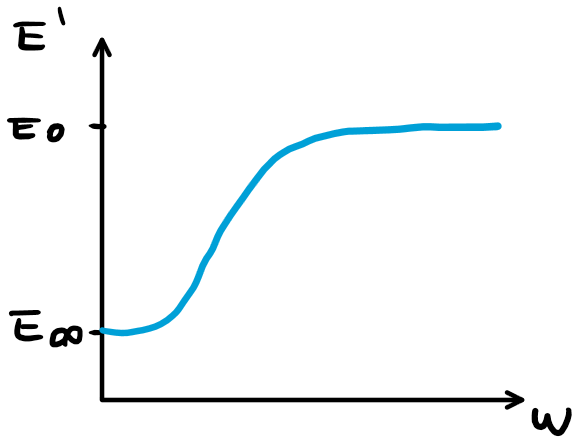
\includegraphics[width = 0.4\textwidth]{gfx/Conservativa3Param}}\quad
\subfloat[][\emph{Componente dissipativa per il modello a tre parametri}\label{fig:Dissipativa3Param}]
{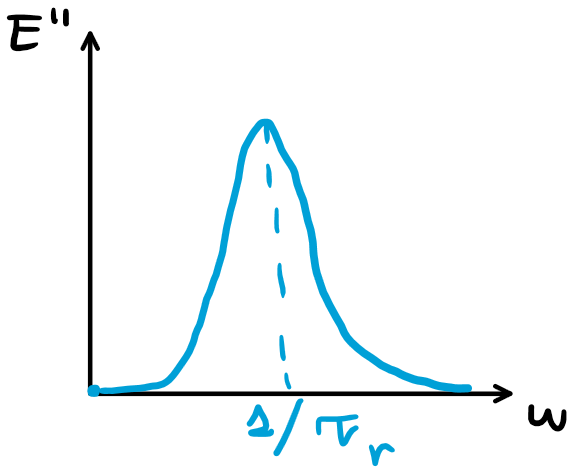
\includegraphics[width = 0.4\textwidth]{gfx/Dissipativa3Param}}
\caption{Risultati di un prova dinamica per un fluido a tre parametri}
\label{fig:3Param}
\end{figure}
Il tempo di rilassamento è tale per cui il materiale posto a deformazione a frequenze pari all'inverso del tempo di rilassamento. presenta la massima dissipazione.